\documentclass[12pt]{article}

\usepackage{graphicx}
\usepackage{float}
\usepackage{amsmath}
\usepackage{amssymb}
\usepackage{graphicx}
\usepackage[utf8]{inputenc}
\usepackage[spanish]{babel}
\usepackage{geometry}
\geometry{left=2cm,right=2cm,top=2cm,bottom=2cm}
\usepackage{listings}
\lstset{basicstyle=\ttfamily,
  showstringspaces=false,
  commentstyle=\color{red},
  keywordstyle=\color{blue}
}


\title{%
  Proyecto 01\\
  \large Motor Grafico \\
    \Large Computación Gráfic4\\
     \large UNAM 2022-2}
\author{Gibran Zazueta Cruz \\
\small 21/abril/2022}
\date{}

\begin{document}
\maketitle

\section{Introducción}

El programa que se presenta a continuación implementa el renderizado de una malla 3d utilizando un método de rasterización. 

Se implementa
\begin{itemize}
\item Lectura de archivos wavefront OBJ

\item Proyección de vértices 3d a coordenadas del dispositivo

\item Cálculo de normales

\item Scan Conversion

\item Sombreado de Phong y gouroud

\item Texturizado sobre caras específicas


\end{itemize}

\section{Leer malla 3d}

Se toma la información de los vértices y normales del mesh desde un archivo formato OBJ.
Para la lectura se utilizó una librearía externa.

\subsubsection{Librería \textit{assimp}}

Para leer los archivos se utiliza la libreria de \text{assimp}. 
\textit{Assimp} es una librería open source que soporta multiples formatos de geometria 3d, entre llos .OBJ. Además funciona con diversos sistemas operativos y provee una interfaz de C++.

También soporta una jerarquía de nodos para mallas, materiales, texturas y animaciones de \textit{bones}. Para el programa de este reporte se hace uso principalmente de la función \textit{import} de la clase Assimp::Importer que almacena datos es una estructura llamada aiScene.



\section{Proyecciòn en perspectiva}

Para lograr la proyección se implementaron las matrices de transformación necesarias. Primero la cámara recibe su posición desde la matriz de transformación mundo-cámara.


\begin{equation}
\begin{bmatrix}
M_{c}^{T} &  M_{c}^{T}o_{w}\\
O^{T} & 1 

\end{bmatrix}
\end{equation} 

Donde $M_{c}^{T} $ son los vectores unitarios del marco de la cámara y $o_{w}$ es el desplazamaiento con respecto al mundo.
Para las dos vistas de las cámaras utilizadas en la escena resultan las siguientes matrices:

$$
M_{camara1}= \begin{bmatrix}
1 & 0 & 0& 0\\
0 & 1 & 0& 0\\
0 & 0 & 1&-2 \\
0 & 0 & 0&1
\end{bmatrix}
M_{camara2}= \begin{bmatrix}
0.86 & 0 & 0.5& 0\\
0 & 1 & 0& 5\\
-0.5 & 0 & 0.86&-2 \\
0 & 0 & 0&1
\end{bmatrix}
M_{camara3}= \begin{bmatrix}
-1 & 0 & 0& 0\\
0 & 1 & 0& 0\\
0 & 0 & -1&-2 \\
0 & 0 & 0&1
\end{bmatrix}
$$


Por otro lado, el espacio del dispositivo tiene las dimensiones de 400x400 px y un sistema de coordenadas como se muestra en la figura

\begin{figure}[H]
\centering
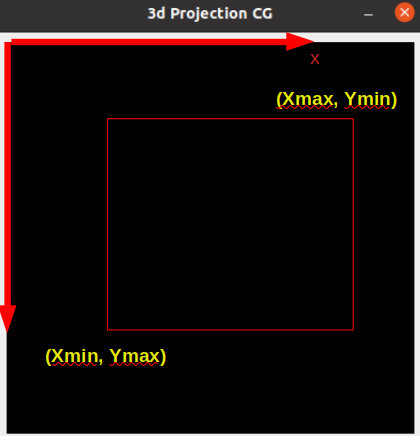
\includegraphics[scale=0.45]{images/axis.png}
\caption{Ejes del plano del dispositivo}
\label{axis}
\end{figure}


\section{Scan Conversion}

A continuaciòn se explica el método de scan conversion 


Para lograr rellenar un polígono primero se almacena la información de sus aristas en un \textit{Buffer}.


\begin{figure}[H]
\centering
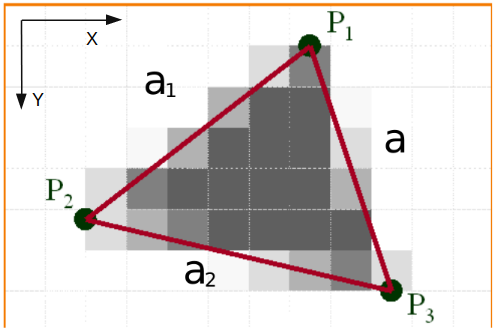
\includegraphics[scale=0.5]{images/scanfillED.png}
\caption{Algortimo rellenado de poligonos con Scan Conversion (imagen obtenida de \cite{fill})}
\end{figure}

Se siguen las aristas de la figura, una por una. Se calcula la pendiente de la recta y se va avanzando una unidad (de pixel) por \textit{y}, calculando el valor correspondiente para \textit{x}. Este proceso se debe realizar en orden, es decir, las aristas se siguen en orden horario o antihorario. 

Tomando como ejemplo la figura 2, un procesamiento antihorario sería: $a_{1} \rightarrow a_{2} \rightarrow a_{3}$.\\

La idea es dividir las aristas del polígono entre un 'lado izquierdo' y un 'lado derecho' que permita colorear los pixeles desde un borde hasta el otro, por cada coordenada $y$. 
Con un procesamiento de este tipo y para un polígono convexo el buffer almacenará 2 coordendas de $x$ por cada coordenada de $y$.\\

La manera en que se clasifican los bordes, entra parte derecha e izquierda, es tomando en cuenta el valor menor entre los dos vértices que forman la arista (por ejemplo $P_{1_{y}}$ y $P_{2_{y}}$ para la arista $a_{1}$).

Para un recorrido antihorario, mientras el valor del primer punto de la arista sea menor al del segundo se considera que esta pertenece al lado izquierdo. Cuando el valor del segundo punto de la arista sea menor al primero, la recta pertenece al lado derecho. 

La información de las coordendas $x$ (derecha e izquierda) correspondientes a cada coordenada $y$ se almacena en el buffer.\\

Una vez se tiene la información del buffer, se recorre la figura de arriba hacia abajo (tomando en cuenta el eje de coordenadas del dispostivo, esto corresponde a un incremento en  $y$), donde por cada valor de $y$ se colorean los pixeles desde la coordenada $x$ derecha hasta la $x$ izquierda.

Esta implementación está basada en la información presentada en \cite{bb}


\section{Shading}
Para el sombreado su utilizan el mètodo de sombreado de Phong 

El modelo de iluminación de Phong presenta las siguientes ecuaciones de sus componentes ambental, difusa y especular.

\textit{Ambiental}

Se calcula como

\begin{equation}
I_{A}=\kappa_{A}\Lambda_{A}
\end{equation}

La luz \textit {difusa} se calcula como 

\begin{equation}
I_{D}=\kappa_{D}\Lambda_{D}(\vec{n} \cdot \vec{l})
\end{equation}

\textit{Especular}
El calculO es el siguiente

\begin{equation} \label{eq:3}
I_{E}=\kappa_{E}\Lambda_{E}(\vec{o} \cdot \vec{l})^{\rho}
\end{equation}

donde $\vec{o}$ es el vector de dirección del observador. La ecuación (3) también se puede escribir

\begin{equation}
I_{E}=\kappa_{E}\Lambda_{E}(\vec{o} \cdot \vec{h})^{\rho}
\end{equation}


donde $h=2(\vec{o} \cdot \vec{l})\vec{n}-\vec{l}$

\subsection{Materiales y Escena}
Los objetos cuentan con 2 posibles materiales a seleccionar, estos se definen dentro del código como:

\textbf{Material 1}
\begin{itemize}
\item Ambiental = {0.0, 0.0, 0.0, 1.0},
\item Difusa = {0.50, 0.50, 0.50, 1.0},
\item Especular {0.70, 0.70, 0.70, 1.0} 
\item $\rho$ = 32.0.
\end{itemize}


\textbf{Material 2}
\begin{itemize}
\item Ambiental = {0.23125, 0.23125, 0.23125, 1.0},
\item Difusa = {0.2775, 0.2775, 0.2775, 1.0},
\item Especular {0.773911, 0.773911, 0.773911, 1.0}
\item $\rho$ = 89.6.
\end{itemize}


Finalmente, la escena a renderizar cuenta con 2 luces (blanca y azul) y 3 cámaras.

Se disponen de la siguiente manera: 

\begin{figure}[H]
\centering
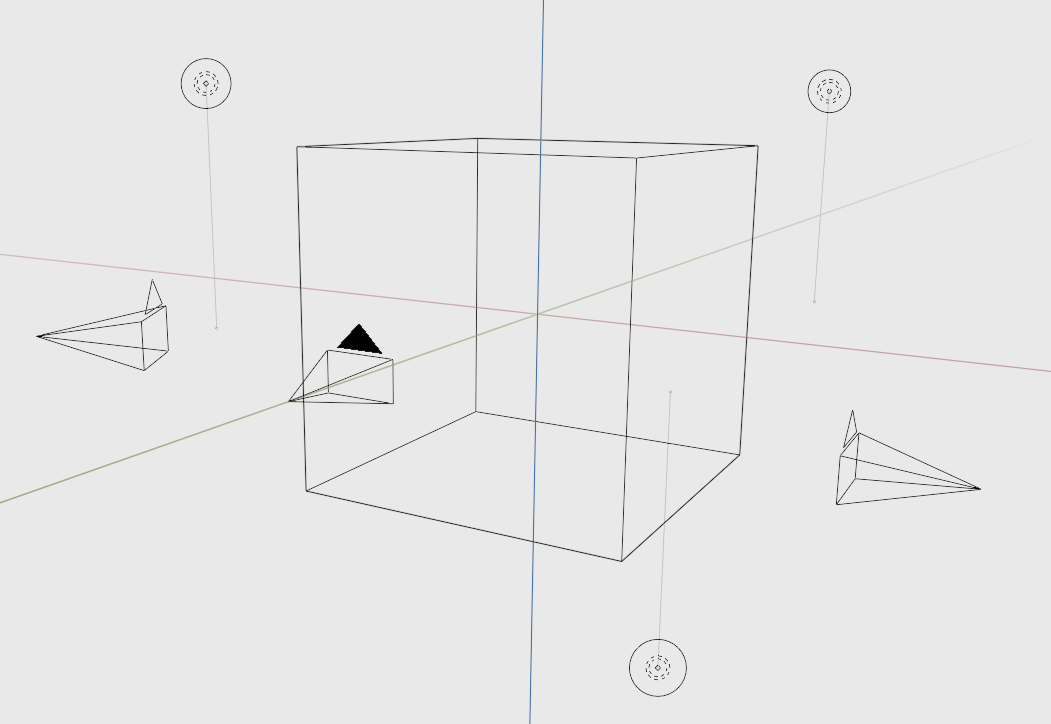
\includegraphics[scale=0.6]{images/escena.png}
\caption{Posición de las componentes de la escena}
\end{figure}



\subsection{Texturas}

El mapeo de texturas consiste en realizar un mapeo de coordenadas (u,v) de una imagen a las coordenadas de la cara de un polígono. El propósito es aplicar un sombreado por medio de una imagen 2d.

El mapeo de texturas utilizado es un mapeo afín, es decir no toma en cuenta la perspectiva. Esto ocasiona un efecto como el mostrado en la figura

\begin{figure}[H]
\centering
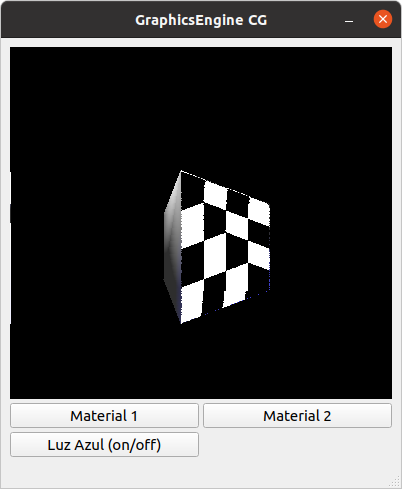
\includegraphics[scale=0.5]{images/afin.png}
\caption{Mapeo afin}
\end{figure}


Las texturas utilizadas para los materiales 1 y 2 son:



\begin{figure}[H]
\centering
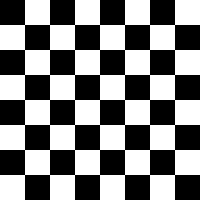
\includegraphics[scale=3]{images/textura2.png}
\caption{Textura material 1}
\end{figure}

\begin{figure}[H]
\centering
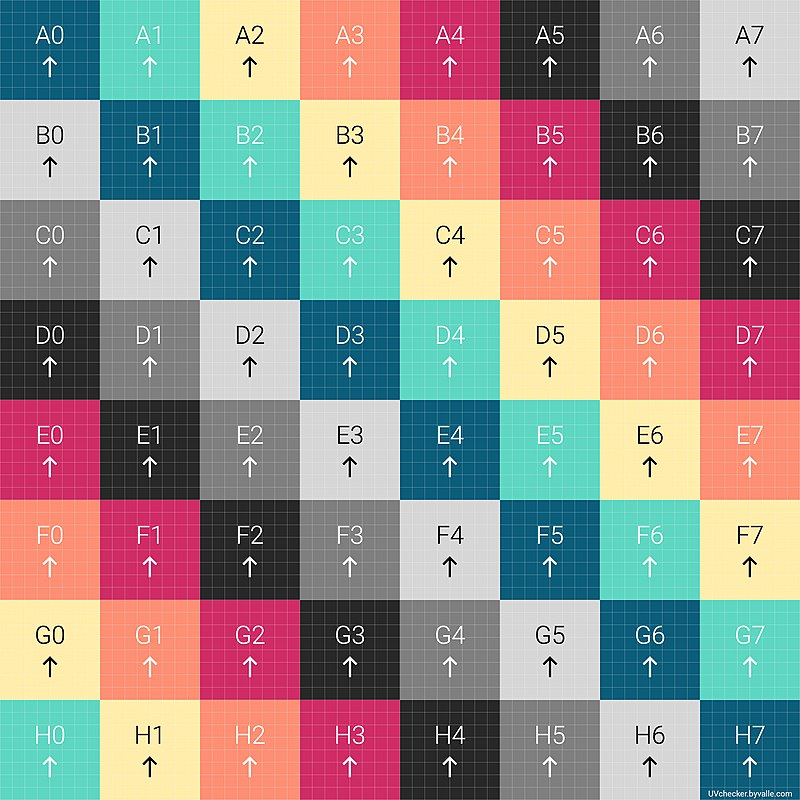
\includegraphics[scale=0.2]{images/textura1.jpg}
\caption{Textura material 2}
\end{figure}



Sobre el objeto del conejo, la textura solo se visualiza en una parte correspondiente a 72 caras (triángulos) de la malla.




\section{Estructura del código}


 \subsection{CubeObject}
Almacena la informaciòn del objeto a renderizar. Esto incluye coordenadas de los vertices, definición de las caras del poligono (por medio de indices a los vertices), normales de las caras, normales de los vértices, coordenadas UV e informaciòn sobre el material (coeficientes ka,kd,ke)

En el constructor de la clase de definen los 2 materiales a utilizar. En los materiales también se puede cargar una textura, correspondiente a ese material.

Esta clase también tiene mètodos para realizar rotaciòn de euler en $x$, $y$ y $z$, y para calcular las normales de las caras y de los vértices. La información de las normales también se puede almancenar desde un archivo OBJ

\subsection{raster}
\textit{raster} es la clase más importante ya que en su mètodo pipeline se realiza la proyección, scan conversion y sombreado

Para la proyección se utliza la clase \textit{\textbf{camProjection}}. En el método \textit{projectPoint} de esta clase se realiza proyección en perspectiva u ortogonal, además se mapea a coordenadas del dispositivo. De este método se obtienen estas coordenadas e información de profundidad

Después se calcula en los vértices los valores para los vectores de normales (N), posición de luz (L) y observador (O). Con estos se pueden calular el valor de color en los vértices (ùtil para realizar la interpolaciòn de sombreado de gouroud), o se pueden interpolar para, posteriormente, obtener el sombreado de Phong.

A continuación, con el método \textit{fillCubeFace}, se utiliza el aloritmo de scan conversion descrito anteriormente para rellenar los pixeles del polígono y a su vez para interpolar N,L,O, Color, profundidad y coordenadas de textura 

la primera interpolaciòn sobre los bordes se realiza con el método \textit{scanline}. Se busca aplicar scanline entre todos los vèrtices del polìgono. Posteriormente se realiza la interpolaciòn horizontal, para ello se utilizan las funciones \textit{scanConversion} y \textit{horInterpolation}

EN el caso de que se requiera dibujar textura, es en este método que se recupera la información de la imagen solo para las caras que asi lo requieran

\subsection{lights}
La clase \textit{lights} almacena la informaciòn de las luces de la escena. Se define su intensidad, color y posiciòn

\subsection{renderwindow}

Se utiliza la biblioteca de \textbf{qt} para pintar sobre el canvas. Al dibujar un pixel se toma en cuenta la profundidad interpolada (o mas bien el inverso 1/z).
El punto solo se dibujarà en el canvas si no existe otro pixel en la misma posición con profundidad menor (es decir, un pixel que ocluya al anterior)

\subsection{mainWindow}
Desde \textit{mainwindow.cpp} se llama a la función \textit{importFile()} que está definida en \textit{functions.cpp}. La función recibe el path del archivo (como una cadena std::string) y apuntadores al contenedor de vertices y caras del objeto cubeObject,

Después de esto, en mainwindow se crean los objetos de clase \textit{light} para las luces blanca, azul y especular, se especifican intensidad, color y posicionamiento. También se crea el grid de botones que conforma la GUI de la aplicacion. Finalmente se llama a la funcion \textit{drawObject()}

En la funcion  \textit{drawObject()} se llama a la función pipeline del objeto raster, que como ya se mencionó relaza todo lo referente a la proyección, rellenado y sombreado.


\section{Ejecutar el programa}
En la carpeta de build se puede ejecutar el programa con el archivo GraphicsEngine-Run. Desde la consola de comandos de linux:

\begin{lstlisting}[language=bash,title={bash}]
./GraphicsEngine-Run
\end{lstlisting}


En la carpeta principal está el código fuente. Para generar el ejecutable primero se genera el Makefile con

\begin{lstlisting}[language=bash,title={bash}]
 qmake GraphicsEngine.pro
\end{lstlisting}

Después se construye el proyecto con \textit{make}



\section{Instrucciones de uso}
Se presenta la interfaz del programa.

\begin{figure}[H]
\centering
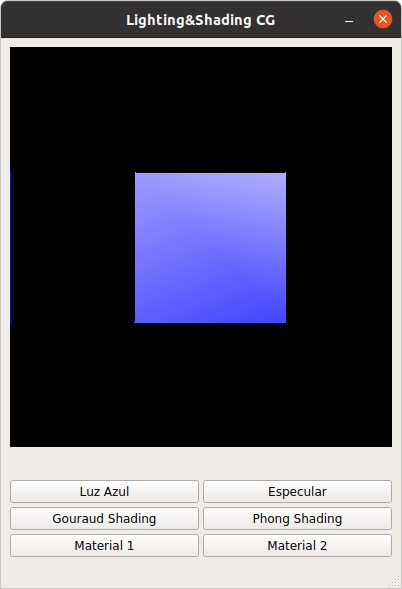
\includegraphics[scale=0.5]{images/ej1.png}
\caption{Interfaz gráfica del programa}
\end{figure}

Para cambiar entre las camaras se utilizan las teclas de los numeros
\begin{itemize}
\item "1". Cambia a la cámara 1
\item "2". Cambia a la cámara 2
\item "3". Cambia a la cámara 3

\end{itemize}

 

Se puede rotar el objeto $30º$ sobre el eje $y$. Para hacerlo se presiona la tecla R del teclado.
\\

El programa incia con luz blanca y luz azul activa. La luz azul se puede deshabilitar al presionar el botòn \textit{Luz Azul (on/off)}
\\


Es posible cambiar entre archivos desde el código. En la variable path de mainwindow se cambia la extension por el archivo correspondiente. Por defecto es $bunny$, los demàs archivos se encuentra en la carpeta $'object\_file'$ del proyecto.

Tambièn se puede cambiar la posiciòn de las càmaras al modificar las matrices dentor de la función \textbf{pipeline} dentro de \textit{raster.cpp}. De igual manera, la posición de las luces, que fue definida en \textit{mainwindow.cpp}


\section{Resultados}

El programa se corriò en un computadora con procesador AMD FX-8370, con tarjeta gráfica Nvidia GTX 970 y 12 gb de memoria ram. El conejo se renderizó en un tiempo aproximado de 14 minutos.

\begin{figure}[H]
\centering
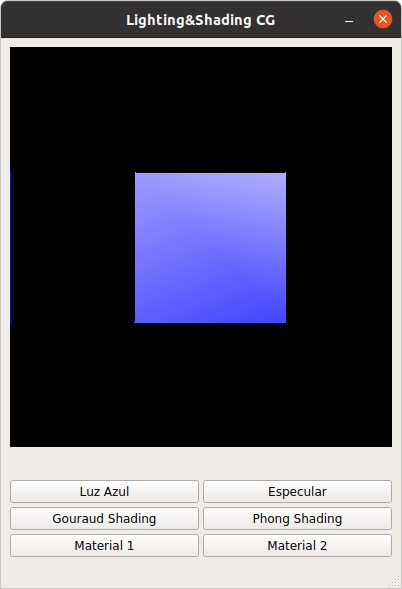
\includegraphics[scale=0.5]{images/ej1.png}
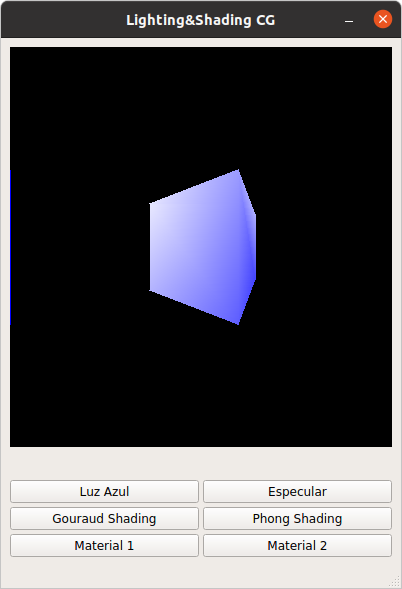
\includegraphics[scale=0.5]{images/ej2.png}
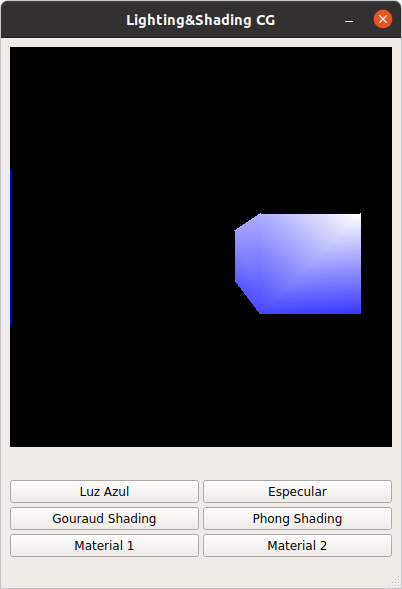
\includegraphics[scale=0.5]{images/ej3.png}
\caption{Renderizado de cubo con Phong y textura}
\end{figure}


\begin{figure}[H]
\centering
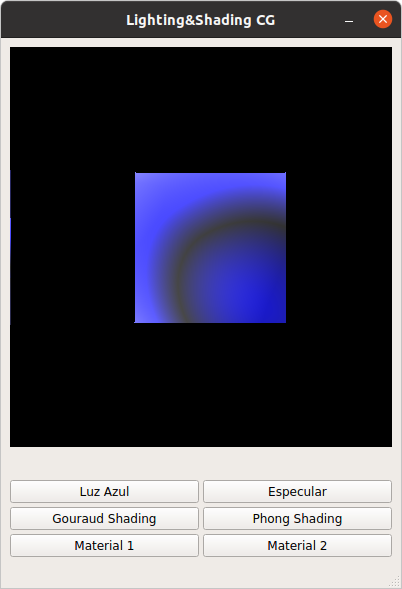
\includegraphics[scale=0.5]{images/ej4.png}
\caption{Renderizado de conejo. Càmara 1. Material 2}
\end{figure}

\begin{figure}[H]
\centering
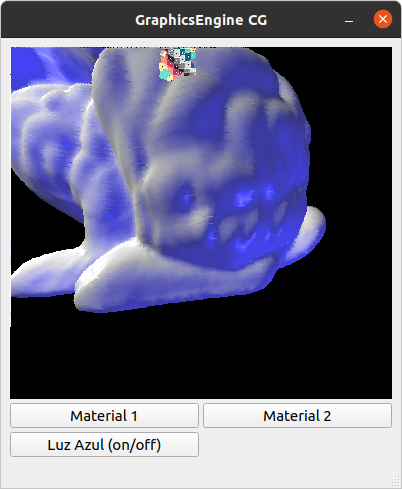
\includegraphics[scale=0.5]{images/ej5.png}
\caption{Renderizado de conejo. Càmara 2. Material 2}
\end{figure}




\begin{thebibliography}{99}

\bibitem{bb} Upssala Universit. Introduction to polygons. ($http://www.it.uu.se/edu/course/homepage$\\$/grafik1/ht06/Lectures/L02/LinePolygon/x_polyd.htm$)
\end{thebibliography}

\end{document}